\newpage
\hypertarget{allCards tex}{}
\subsection{AllOtherCardsRule}
\texHeader

\begin{itemize}

\item[$\blacktriangleright$] Right click on the \texttt{Rules} folder again and create \texttt{AllOtherCardsRule}. Complete each scope until your file resembles
Fig.~\ref{eclipse:allOtherCardsRuleComplete}.

\vspace{0.5cm}

\begin{figure}[htbp]
\begin{center}
  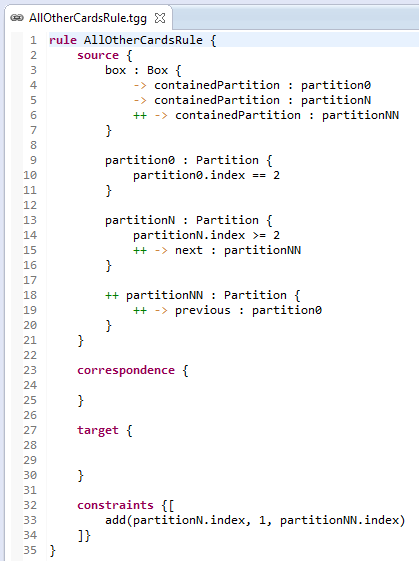
\includegraphics[width=0.6\textwidth]{eclipse_AllOtherCardsRule}
  \caption{A complete \texttt{AllOtherCardsRule}}
  \label{eclipse:allOtherCardsRuleComplete}
\end{center}
\end{figure}

\item[$\blacktriangleright$] You'll notice that \texttt{box} and \texttt{partition0} have been established as `black' objects. This is so the rule may only be
evaluated when these objects are already translated, so we can use their values from the context of the transformation.

\vspace{0.5cm}

\item[$\blacktriangleright$] A second partition, \texttt{partitionN}, has also been established as part of the context. It represents the \texttt{n}th, or last
translated partition in a \texttt{box} (with an index of 2 or higher), whose \texttt{next} reference will also be translated in order to provide an access
link to the new \texttt{partitionNN} element.

\newpage

\item[$\blacktriangleright$] Given that the syntax of \texttt{add(a,b,c)} is \texttt{a+b=c}, the sole constraint of this rule sets the \texttt{index}
of the \texttt{n+1}th partition so that the \texttt{partition}s are still listed in order. Note that the correspondence and target scopes are empty, which is typical
for such ignore rules.

\vspace{0.5cm}

\item[$\blacktriangleright$] That's it! Save and build, then run the TGG again with the `extra' \texttt{partition} to confirm it worked!
If so, you are now free to add as many \texttt{partition}s and \texttt{card}s to \texttt{source.xmi} -- the transformation is now able to elegantly ignore them all.

\vspace{0.5cm}

\item[$\blacktriangleright$] Be sure to check out how this rule is implemented in eMoflon's visual syntax in Fig.~\ref{fig:ea_allOtherCardsRuleComplete} from
the previous section.

\end{itemize}
